% Created 2019-07-31 mi. 12:26
% Intended LaTeX compiler: pdflatex
\documentclass[a4paper,12pt,oneside]{book}
\usepackage[main=spanish, english, ]{babel}%paquete para el idioma del documento. Si
%se quiere utilizar un parrafo con idioma diferente podemos utilizar
%la orden  electlanguage{}
\usepackage[utf8]{inputenx}
\usepackage[T1]{fontenc}
\usepackage{lmodern,pifont}
\usepackage{pdflscape}
\usepackage{caption}
\usepackage{textcomp}
\usepackage{graphicx}
\usepackage{grffile}
\usepackage{wrapfig}
\usepackage{capt-of}
\usepackage[normalem]{ulem} 
\usepackage[dvipsnames]{color}
\usepackage{colortbl}
\usepackage{longtable}
\usepackage{hyperref}
\hypersetup{bookmarksopen,bookmarksnumbered,bookmarksopenlevel=4,%
  linktocpage,colorlinks,urlcolor=black,citecolor=ForestGreen,linkcolor=black,filecolor=black}
\usepackage{natbib}
\usepackage{amssymb}
\usepackage{amsmath}
\usepackage{geometry}
\geometry{a4paper,left=2cm,top=2cm,right=2.5cm,bottom=2cm,marginparsep=7pt, marginparwidth=.6in}


\newcommand{\recuerda}[1]{\begin{center}\fbox{\parbox{0.75\textwidth}{\textbf{Recuerda:}#1}}\end{center}}
\date{}
\title{UF0009. Mantenimiento, preparación y manejo de tractores}
\hypersetup{
 pdfauthor={Antonio Soler Gelde. IT Forestal},
 pdftitle={UF0009. Mantenimiento, preparación y manejo de tractores},
 pdfkeywords={},
 pdfsubject={},
 pdfcreator={Antonio Soler Gelde}, 
 pdflang={Spanish}}
\begin{document}

\maketitle
\thispagestyle{empty} \tableofcontents \clearpage\chapter{El tractor y equipo de tracción}
\label{sec:org951d398}
\section{Definición}
\label{sec:org3d60fc4}
Un tractor, agrícola o forestal, es un vehículo autopropulsado de dos o más
ejes, concebido para arrastrar o empujar aperos, maquinaria o vehículos
agrícolas. 
Otras características generales son:
\begin{itemize}
\item Es capaz de suministrar un gran esfuerzo de tracción (capacidad de tirar
grandes fuerzas en relación a su peso)
\item Puede desplazarse por lugares donde la adherencia no es buena
\item Tiene por diseño una velocidad máxima de desplazamiento de 40 \emph{km/h}
\end{itemize}
\section{Constitución del tractor}
\label{sec:org7749cba}
Aunque hay mucha diversidad en el diseño de tractores se pueden distinguir una
serie de partes fundamentales:
\begin{itemize}
\item \textbf{Bastidor:} Armazón metálico sobre el que se sujetan las diferentes partes de
un tractor
\item \textbf{Motor:} Órgano principal que proporciona el movimiento del tractor y el
funcionamiento de los diferentes sistemas
\item \textbf{Transmisión:} Elementos que transmiten la energía generada en el motor hasta
las ruedas y otros dispositivos (toma de fuerza, sistema hidráulico,\ldots{})
\begin{itemize}
\item \textbf{Embrague:} Dispositivo que transmite o interrumpe el giro del motor al
resto de la transmisión
\item \textbf{Caja de cambios:} Conjunto de engranajes que permiten adecuar la velocidad
del tractor
\item \textbf{Diferencial:} Mecanismo que permite que dos ruedas tengan diferentes
velocidades de giro y pueda tomar las curvas con facilidad
\item \textbf{Reductora:} Mecanismo que aumenta la fuerza de tracción modificando la
velocidad de giro de las ruedas
\item \textbf{Palieres:} Ejes que transmiten el movimiento desde el diferencial hasta las ruedas
\end{itemize}
\item \textbf{Ruedas:} Elementos sobre los que se apoya todo el peso del tractor y le
permiten desplazarse
\item \textbf{Elevador hidráulico:} Elemento que permite elevar o descender los aperos
acoplados al tractor
\item \textbf{Enganche tri-puntal:} Mecanismo en el que se acoplan los aperos del tractor
y se accionan mediante la toma de fuerza
\item \textbf{Dirección:} El conjunto de piezas que sirven para dirigir al tractor. Actúa
sobre las ruedas delanteras llamadas ruedas directrices
\item \textbf{Frenos:} Los encargados de disminuir la velocidad del tractor e incluso
detenerlo completamente
\end{itemize}

\begin{figure}[htbp]
\centering
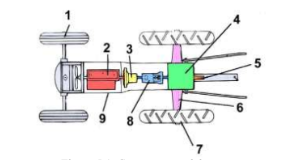
\includegraphics[width=0.8\textwidth]{./img_0009/tractor_partes.PNG}
\caption{Componentes del tractor}
\end{figure}

\begin{enumerate}
\item Ruedas directrices
\item Motor
\item Embrague
\item Diferencial
\item Toma de fuerza
\item Palier y reducción final
\item Ruedas motrices
\item Caja de cambios y grupo reductor
\item Bastidor
\end{enumerate}
\section{Trabajos que puede realizar}
\label{sec:org4a743ca}
El tractor es una máquina que tiene diferentes aplicaciones en agricultura y
selvicultura. Los diferentes trabajos que realiza los podemos clasificar en:
\begin{itemize}
\item \textbf{Estacionarios}.
\begin{itemize}
\item Mediante la toma de fuerza, por ejemplo accionar una bomba de riego
\item Mediante el sistema hidráulico, por ejemplo accionar un elevador de grano
\end{itemize}
\end{itemize}
\begin{center}
\begin{figure}[htbp]
\centering
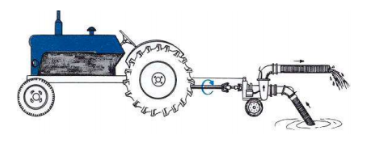
\includegraphics[width=0.6\textwidth]{./img_0009/tractor_riego.PNG}
\caption{Accionando una bomba de riego}
\end{figure}
\end{center}
\begin{itemize}
\item \textbf{De transporte}. Por ejemplo tirar un remolque
\end{itemize}
\begin{center}
\begin{figure}[htbp]
\centering
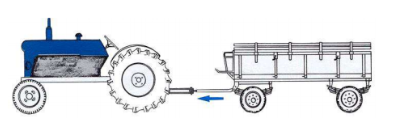
\includegraphics[width=0.6\textwidth]{./img_0009/tractor_remolque.PNG}
\caption{Transportando un remolque}
\end{figure}
\end{center}
\begin{itemize}
\item \textbf{De arrastre}. Por ejemplo tirar de un arado
\end{itemize}
\begin{center}
\begin{figure}[htbp]
\centering
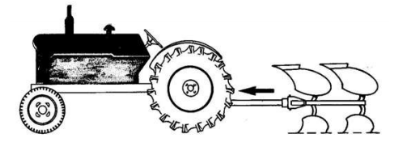
\includegraphics[width=0.6\textwidth]{./img_0009/tractor_arado.PNG}
\caption{Arrastrando un arado}
\end{figure}
\end{center}
\begin{itemize}
\item \textbf{De empuje}. Por ejemplo trabajar con una pala cargadora
\end{itemize}
\begin{center}
\begin{figure}[htbp]
\centering
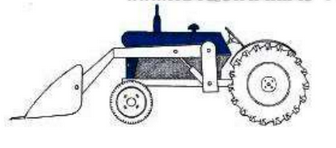
\includegraphics[width=0.6\textwidth]{./img_0009/tractor_pala.PNG}
\caption{Accionando una pala}
\end{figure}
\end{center}
\begin{itemize}
\item \textbf{Combinados}
\begin{itemize}
\item Transporte y toma de fuerza. Por ejemplo remolque accionado
\item Arrastre y toma de fuerza. Por ejemplo llevar una fresadora
\end{itemize}
\end{itemize}

Todas estas posibilidades se resumen en 4 grandes acciones que constituyen las
aplicaciones básicas del tractor:
\begin{itemize}
\item Remolcar
\item Arrastrar
\item Empujar
\item Transmitir movimiento
\end{itemize}
\section{Sistema de tracción del tractor}
\label{sec:org8ad5ab6}

Podemos dividir el sistema de tracción de un tractor típico en las siguientes
partes:
\begin{enumerate}
\item \textbf{Motor y sus componentes}
\label{sec:org381c5d5}

Cilindros, bielas, cigüeñal,etc.

\item \textbf{Transmisión}
\label{sec:orgc95c2a0}

Formada por el embrague (separa el motor de la transmisión), cambio de
velocidades y el diferencial (comunica el giro del motor a las ruedas
propulsoras).
\item \textbf{Dirección}
\label{sec:orgaacdad8}

Se maneja a través del volante por el conductor, dirige a un lado o a otro las
ruedas.
\item \textbf{Mecanismos auxiliares}
\label{sec:org43c826d}

Frenos, sistema eléctrico,sistema de refrigeración, ruedas, sistema eléctrico,
etc.
\end{enumerate}

\section{El motor}
\label{sec:org32b16f9}

El motor proporciona la potencia y el rendimiento del tractor.  Está situado en 
la parte delantera del mismo cubierto por el capó.
\begin{center}%
\fbox{\parbox{0.6\textwidth}{\textbf{Recuerda:}  El combustible que utilizan
los motores de tractor es \textbf{diésel.}}}
\end{center}

Visualmente podemos dividir al motor en tres partes:
\begin{itemize}
\item \textbf{Bloque motor:} es la parte central del motor donde van alojados diferentes
partes como pistones, cigüeñal, volante de inercia, etc
\item \textbf{Tapa de culata y balancines:} situado en la parte superior del bloque
motor. es la parte que canaliza los gases producidos por la combustión del carburante
\item \textbf{Cárter:} situado en la parte inferior del bloque motor. Recoge el aceite del
sistema de engrase para ser enviado a las partes móviles del motor
\end{itemize}

\begin{figure}[htbp]
\centering
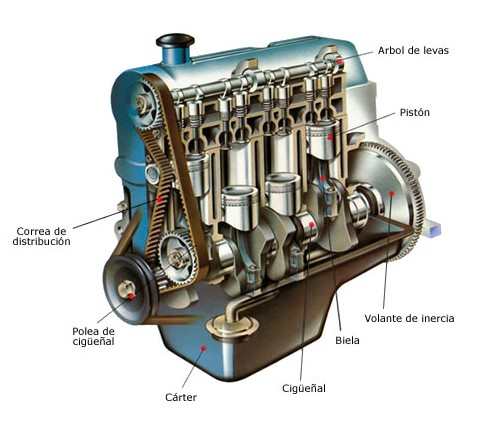
\includegraphics[width=0.8\textwidth]{./img_0009/motor_1.jpg}
\caption{Partes de un motor de cuatro tiempos}
\end{figure}
\vspace{2cm}
\subsection{Componentes internos del motor}
\label{sec:org6daad88}

\begin{itemize}
\item \textbf{Cilindros:} situados en el bloque del motor. Son los tubos huecos por donde
se mueven los pistones
\item \textbf{Pistones:} piezas móviles expuestas a la combustión del combustible. Realizan
un movimiento alternativo y están unidos a  las bielas para transmitir el
movimiento al cigüeñal
\item \textbf{Anillos:} situados alrededor del pistón muy próximos a la cabeza del
mismo. Su misión es que no se produzcan perdidas de gases en el cilindro
\item \textbf{Bielas:} unidas por un extremo a los pistones y por otro al
cigüeñal. Transmiten el movimiento generado por la combustión del combustible
\item \textbf{Cigüeñal:} transforma el movimiento alternativo del pistón en movimiento
rotatorio. Este movimiento rotatorio es el que hace que, además que el
tractor se desplace, funcionen los sistemas de engrase, encendido,
lubricación, toma de fuerza.
\item \textbf{Volante de inercia:} almacena la energía para que el pistón pueda volver a la
parte superior del cilindro
\item \textbf{Válvulas:} permiten la entrada y salida de gases del cilindro. Se disponen de
dos en dos (como mínimo) en el cilindro, una conectada al colector de entrada
de gases y otra al colector de salida
\item \textbf{Eje de levas o balancines:} recibe el movimiento del cigüeñal y realiza la
apertura y cierre de las válvulas
\end{itemize}

\begin{figure}[htbp]
\centering
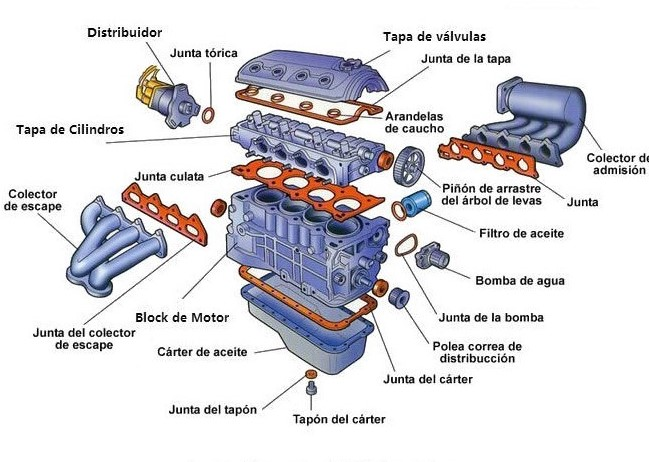
\includegraphics[width=0.9\textwidth]{./img_0009/despiece_motor.jpg}
\caption{Despiece de un motor de 4 cilindros en línea}
\end{figure}
\vspace{2cm}
\subsection{Funcionamiento interno del motor. Los tiempos de funcionamiento}
\label{sec:org84bdf6a}
Los tractores agrícolas y forestales funcionan mediante motores de cuatro
tiempos. Veamos los pasos de funcionamiento que sigue este tipo de motor.

\begin{enumerate}
\item \textbf{Tiempo de admisión:} entrada del aire en el cilindro. Cuando el cilindro
está lleno de aire, el pistón comienza a descender, \uline{se abre la válvula de
admisión} y la válvula de escape se encuentra \uline{cerrada}.
\item \textbf{Tiempo de compresión:} El pistón comienza su carrera ascendente y en ese
momento se \uline{cierra la válvula de admisión} produciéndose de esta manera la
\uline{compresión del aire admitido en el cilindro}
\item \textbf{Tiempo de trabajo o explosión:} se produce la inyección del combustible y combustión del
mismo. Por la elevada presión y temperatura existentes en el cilindro, se
produce la combustión del combustible que empuja al pistón. Las válvulas de
admisión y escape se encuentran cerradas.
\item \textbf{Tiempo de escape:} se expulsan los gases producidos por la combustión.
Debido a la inercia que tiene el cigüeñal el pistón comienza una nueva
carrera ascendente, en ese momento \uline{se abre la válvula de escape}, y el
pistón empuja los gases al colector de escape. La válvula de admisión se 
encuentra cerrada y se abrirá de nuevo al finalizar la carrera ascendente
 para comenzar un nuevo ciclo.
\end{enumerate}
\begin{figure}[htbp]
\centering
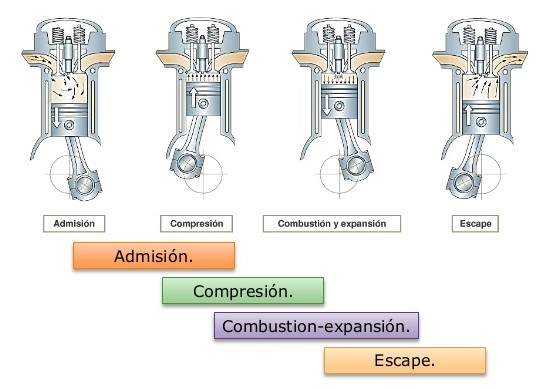
\includegraphics[width=0.8\textwidth]{./img_0009/4tiempos_diesel.jpg}
\caption{Ciclos de un motor de cuatro tiempos}
\end{figure}
\begin{center}%
\fbox{\parbox{0.75\textwidth}{\textbf{Recuerda:}  Los ciclo de trabajo de 
un motor con combustible diesel y gasolína son \textbf{iguales}. La 
diferencia está en que en los motores gasolina se introduce en el cilindro 
una mezcla de \textbf{aire y gasolina}, mientras qué en los diesel es solo 
\textbf{aire} lo que se introduce en el cilindro, el combustible se introduce 
en el cilindro a \textbf{alta presión} mediante los \textbf{inyectores.}}}}
\end{center}

\subsection{Sistema de distribución y admisión}
\label{sec:orgbc9e9a5}
El conjunto de dispositivos necesarios para \uline{regular la entrada y salida de 
gases del cilindro} conforman la \textbf{distribución}.

Los elementos principales que constituyen la distribución son los siguientes:
\begin{itemize}
\item \textbf{Válvulas:} tienen como misión abrir o cerrar los orificios de entrada de
gases al cilindro
\end{itemize}
\begin{figure}[htbp]
\centering
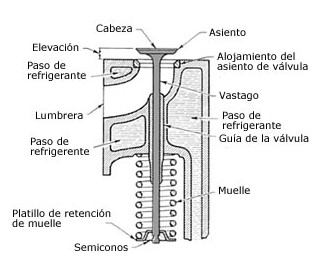
\includegraphics[width=0.5\textwidth]{./img_0009/valvulabloque.jpg}
\caption{Esquema de una válvula y partes de la culata}
\end{figure}
\begin{itemize}
\item \textbf{Eje de levas:} sincronizado con el cigüeñal mediante es el encargado de que las
válvulas se abran o cierren en el momento apropiado
\end{itemize}
\begin{figure}[htbp]
\centering
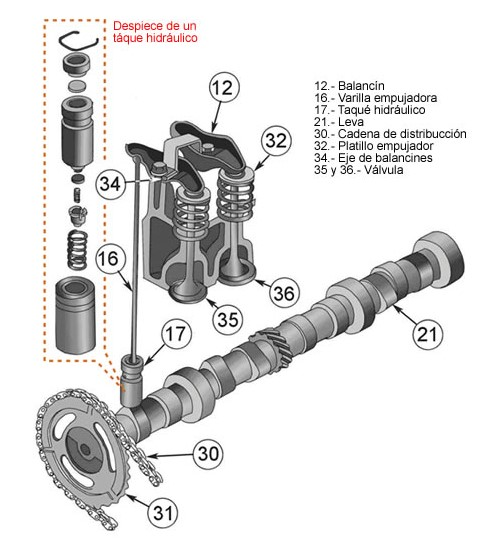
\includegraphics[width=0.5\textwidth]{./img_0009/esquema_distribucion.jpg}
\caption{Detalle de eje de balancies o de levas}
\end{figure}
\begin{itemize}
\item \textbf{Empujadores:} transmiten el empuje del eje de levas a los balancines
\item \textbf{Balancines:} palancas que transmiten el movimiento de las levas a las válvulas
\item \textbf{Correa o cadena de distribución :} correa que transmite el movimiento del
cigüeñal al eje de levas para que este realice su función
\end{itemize}

\begin{center}%
\fbox{\parbox{\textwidth}{Estos elementos actúan en conjunto abriendo y cerrando las válvulas en los
tiempos de admisión y escape de cada cilindro. Esto se ha de realizar de forma
sincronizada con el giro del cigüeñal.}}
\end{center}
\subsection{Sistema de engrase}
\label{sec:org7dde18d}
Un motor de combustión es un conjunto de piezas metálicas que se rozan un as con
otras. Este \uline{rozamiento} produce un gran \uline{desgaste y calentamiento} que puede
llevar a la rotura del motor. Para evitar esto se necesita que las piezas se
deslicen sobre una fina capa de aceite. El conjunto de \uline{piezas y conductos} qué hacen
que el aceite llegue a presión a todas partes se conoce por sistema de engrase o
lubricación. Este sistema consta de:
\begin{itemize}
\item \textbf{Filtro de entrada a bomba:} malla metálica que impide que entre suciedad o
partes metálicas al interior de la bomba evitando su desgaste o rotura
\item \textbf{Bomba de aceite:} recoge el aceite del cárter y lo envía a presión a las
diferentes partes del motor
\item \textbf{Filtro de aceite:} es la pieza encargada de retener las partículas más finas
que contiene el aceite y han pasado por el filtro de entrada a la bomba
\item \textbf{Control de presión:} controla que en todo momento a que presión llega el
aceite a los lugares de engrase. Puede ser un manómetro o un testigo luminoso
\end{itemize}

\begin{figure}[htbp]
\centering
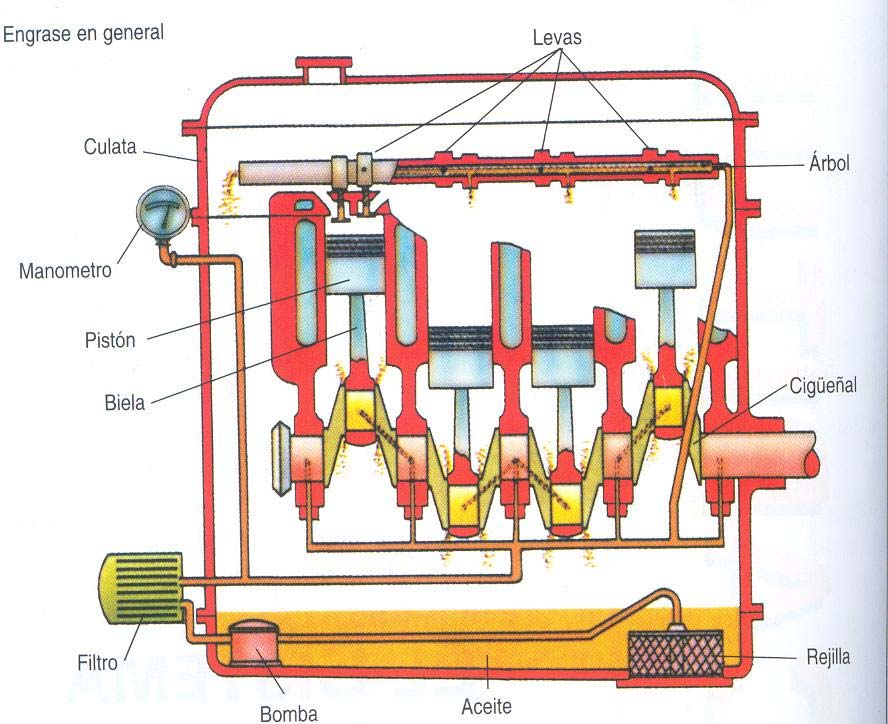
\includegraphics[width=0.65\textwidth]{./img_0009/lubricacion.png}
\caption{Esquema de un sistema de lubricación}
\end{figure}

\subsection{Sistema de refrigeración}
\label{sec:org5d9f306}
En el momento de la combustión se produce un aumento de temperatura que puede
llegar a alcanzar los 1500\textdegree{}C. Esta temperatura podría fundir muchas
piezas , por lo qué se hace necesario \uline{eliminar el exceso de calor} que se
produce, y eso se consigue mediante el sistema de refrigeración.

Existen dos sistemas de refrigeración para motores de combustión, por \uline{aire} y
por \uline{agua o líquida}. 

\begin{itemize}
\item \textbf{Refrigeración por aire:} aprovecha el aire existente alrededor del motor para
enfriarlo. son sistemas típicos de motores 2T. No entraremos en detalle en
ellos ya que no son los sistemas de refrigeración que encontraremos en los
tractores agrícolas o forestales.
\item \textbf{Refrigeración liquida:} un líquido refrigerante es la encargado de enfriar el
motor. Esta  es enfriada por una corriente en el \uline{radiador} y circula a través
de  conducciones por todo el motor. Este sistema cuenta con los siguientes
componentes: 
\begin{itemize}
\item \textbf{Camisa de agua:} cámara hueca que rodea las paredes del cilindro para que
circule el líquido refrigerante
\item \textbf{Radiador:} circuito de tubos en el que se enfría el líquido refrigerante
que viene del motor antes de ser enviado de nuevo. La refrigeración del
liquido suele ser mediante una corriente de aire forzada por un ventilador
que circula a través de unas aletas que están conectadas a los tubos
\item \textbf{Manguitos:} tubos de goma que conectan el radiador con el bloque motor y
otros componentes como el depósito o la bomba
\item \textbf{Bomba de agua:} la que impulsa el líquido refrigerante por el sistema
\item \textbf{Ventilador:} fuerza la entrada de aire a través de las aletas del radiador
\item \textbf{Termostato:} es el encargado de accionar el ventilador cuando la
temperatura del agua se incrementa
\item \textbf{Termometro:} indica la temperatura del líquido refrigerante. Como en el
caso del aceite puede ser un indicador luminoso o de nivel
\end{itemize}
\end{itemize}
\begin{figure}[htbp]
\centering
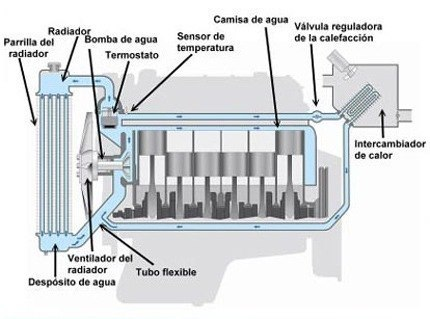
\includegraphics[width=0.55\textwidth]{./img_0009/refrigeracion.jpg}
\caption{Esquema de un sistema de refrigeración}
\end{figure}
\subsection{Sistema de alimentación}
\label{sec:org6031e50}
La característica principal de los motores diésel en comparación con los
gasolina es que el combustible se inyecta en el cilindro y se quema por \uline{aumento 
de la temperatura del aire en el cilindro}. En los motores gasolina es la
\uline{bujía} la encargada de producir una chispa para que el combustible se queme,
\uline{los motores diésel no tienen bujía}.

Para que el combustible diésel llegue al cilindro ha de seguir un recorrido
desde el depósito hasta la cámara de combustión de cada cilindro alojada en la
culata del motor.

Los elementos del sistema de alimentación son los siguientes:
\begin{itemize}
\item \textbf{Deposito:} recipiente en el que se almacena el combustible para el
funcionamiento del motor
\item \textbf{Bomba de alimentación:} es la que aspira el gasóleo del deposito y la envía
con cierta presión al filtro que hay antes de la bomba de inyección
\item \textbf{Filtro de gasoil:} su misión es limpiar el gasoil antes de que llegue a la
bomba de inyección
\item \textbf{Bomba de inyección:} dosifica el combustible y lo envía a través de unas
conducciones a los inyectores en el momento adecuado para que se produzca la
combustión en el cilindro. Está sincronizada con el cigüeñal y la distribución
del motor
\end{itemize}
\begin{figure}[htbp]
\centering
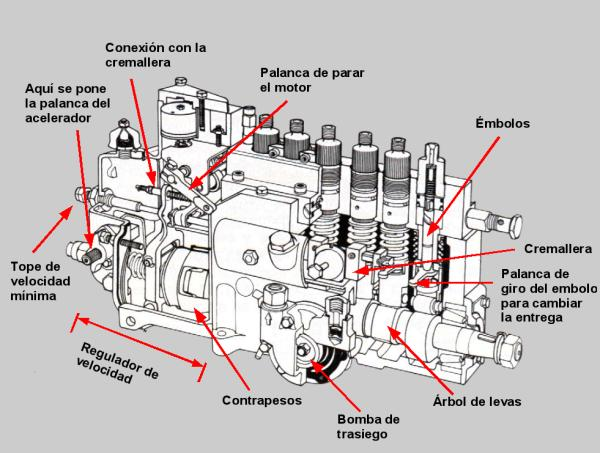
\includegraphics[width=0.5\textwidth]{./img_0009/bomba_inyeccion.jpg}
\caption{Bomba lineal de inyección}
\end{figure}
\begin{itemize}
\item \textbf{Inyectores:} están alojados en la culata del motor. Reciben el combustible a presión desde la bomba de inyección y lo
pulveriza dentro de la cámara de combustión del cilindro
\end{itemize}
\begin{figure}[htbp]
\centering
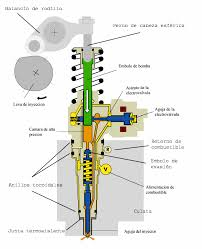
\includegraphics[width=0.45\textwidth]{./img_0009/inyector.jpg}
\caption{Esquema de inyector diesel}
\end{figure}
\newpage

\subsection{Sistema de transmisión}
\label{sec:org4c7e890}
Este sistema hace que el \uline{movimiento de rotación} que se produce en el cigüeñal
pase a la \uline{caja de cambio} mediante el \textbf{embrague} y de ahí a través del
\uline{diferencial} hasta las \uline{ruedas motrices} que dan impulso al tractor.
\begin{enumerate}
\item \textbf{El embrague}
\label{sec:org2d88a4f}

Es el dispositivo por el que se transmite o interrumpe el \uline{movimiento
giratorio} causado por el motor \uline{hacia la caja de cambios}
\begin{center}
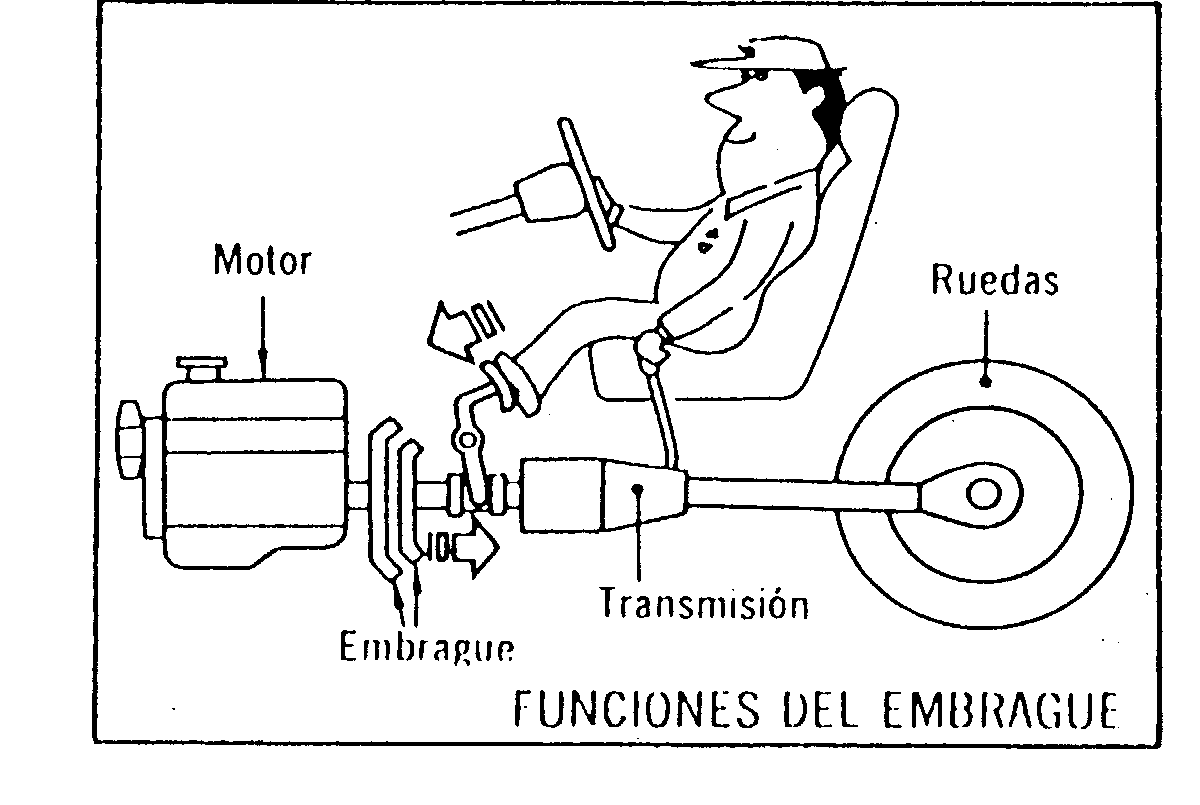
\includegraphics[width=0.5\textwidth]{./img_0009/embrague_1.png}
\end{center}
En esencia, un embrague consta de:
\begin{itemize}
\item \uline{Una tapa metálica o campana} que está unida al volante de inercia y que
encierra en su interior diferentes piezas
\item \uline{Un disco de embrague} que consiste en un disco metálico que lleva en su
parte periférica dos coronas de un material \uline{altamente resistente a la fricción}.
\item \uline{Un disco opresor} del mismo tamaño del disco de embrague, con unas patillas
que actúan sobre el material resistente del disco de embrague
\item Sistema de muelles y resortes que actúan sobre los discos haciendo que estos se
\uline{acoplen y desacoplen} para transmitir el movimiento del motor a la caja de
cambios
\end{itemize}

\begin{figure}[htbp]
\centering
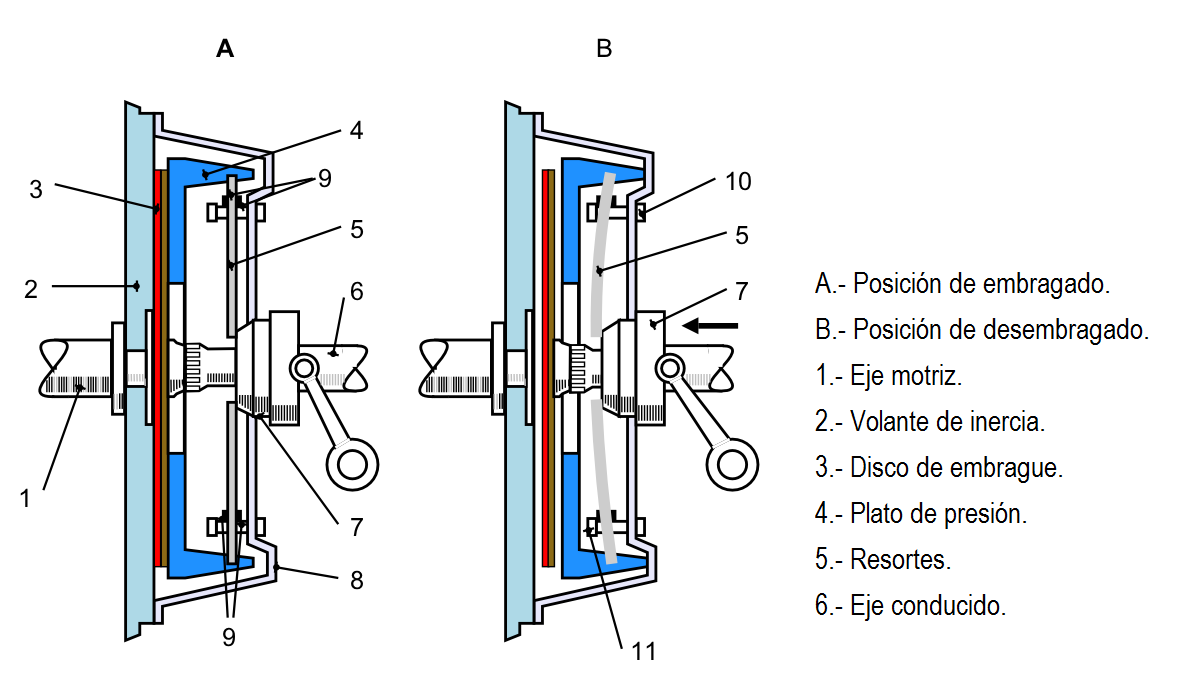
\includegraphics[width=0.55\textwidth]{./img_0009/embrague.png}
\caption{Embrague mono-disco}
\end{figure}

\item \textbf{Caja de cambio}
\label{sec:org2815c7a}

Es el conjunto de ejes y engranajes por los que se logra alcanzar la velocidad
de avance y esfuerzo de tracción adecuado a las necesidades del vehículo.
\begin{figure}[htbp]
\centering
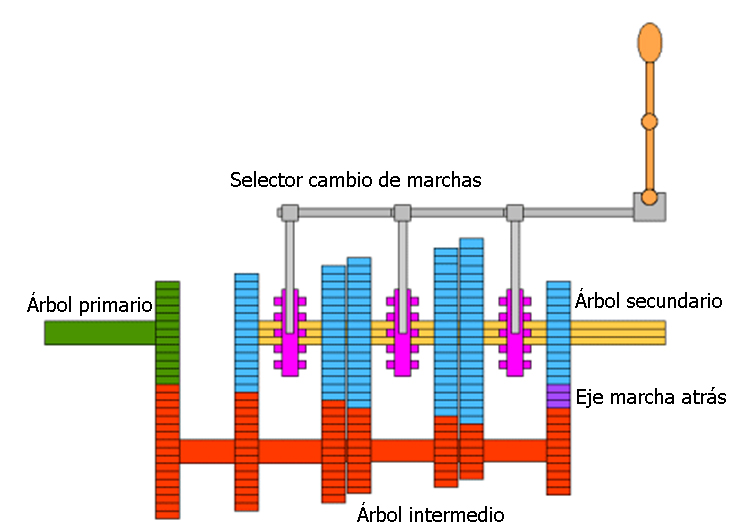
\includegraphics[width=0.65\textwidth]{./img_0009/caja_cambio.jpg}
\caption{Esquema de una caja de cambios}
\end{figure}

La caja de cambio aprovecha al máximo la potencia del motor, adaptando a una
tarea determinada la velocidad de avance del tractor de acuerdo con la fuerza
que requiere para desarrollar cierta labor.

Actualmente los tractores no llevan una única palanca de mando para el cambio de
velocidad, sino \uline{dos o más} para manejar \textbf{la reductora} y la caja de cambios.
\end{enumerate}

\subsection{Toma de fuerza}
\label{sec:org202f569}
Es un eje estriado en su extremo, accionado por el motor del tractor y
\uline{destinado a dar movimiento} a determinado número de máquinas acopladas al
tractor. Esta situado, generalmente, en la parte trasera del tractor.

\begin{figure}[htbp]
\centering
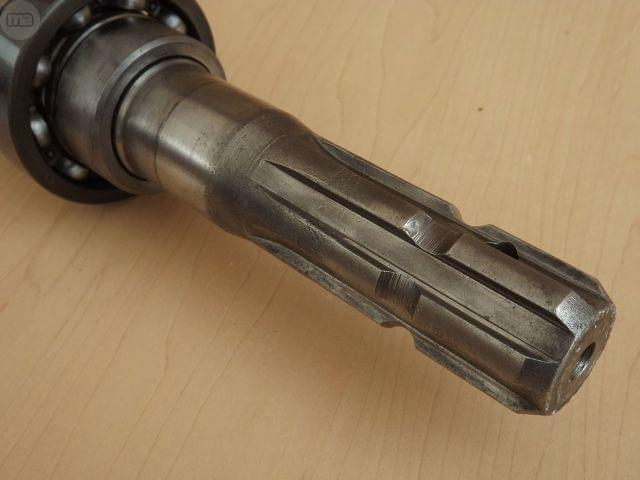
\includegraphics[width=0.45\textwidth]{./img_0009/toma_fuerza_2.jpg}
\caption{Detalle de una barra de toma de fuerza de 540 rpm con 6 estrías}
\end{figure}

La mayoría de los tractores van equipados con una toma de fuerza que gira a 540
\emph{rpm} (revoluciones por minuto) y tienen una conexión exterior con seis estrías
anchas en el eje. 

\newpage
\subsection{Sistema hidráulico}
\label{sec:org56c90d3}
Para acoplar al tractor los aperos agrícolas suspendidos y semi-suspendidos se
emplea el elevador hidráulico.

El elevador hidráulico baja el equipo a la posición de trabajo y lo sube a la
posición de transporte. Tiene dos partes, el enganche a los tres puntos y el
equipo hidrostático.
\begin{figure}[htbp]
\centering
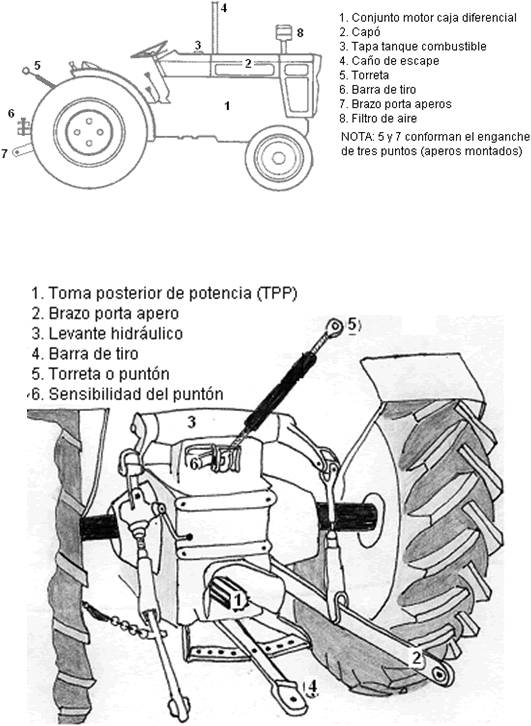
\includegraphics[width=0.65\textwidth]{./img_0009/hidraulico.jpg}
\caption{Esquema de un sistema hidráulico de un tractor con toma de fuerza}
\end{figure}

El enganche a los tres puntos se compone de \uline{dos brazos de tiro rígidos} unidas
al tractor mediante rótulas colocadas en uno de sus extremos, llevando en el
otro extremo sus correspondientes rótulas para el enganche del apero o bien un
\uline{sistema automático:} una barra extensible denominada \textbf{tercer punto}, unida
mediante una rótula al bastidor del tractor y en su extremo lleva otra rótula
para el enganche del apero.
\section{Frenos}
\label{sec:orgab5b4bd}

Son sistemas mecánicos que mediante el rozamiento permiten regular la velocidad
de movimiento, bien disminuyéndola o manteniendola.

Estos frenos pueden ser de dos tipos:
\begin{enumerate}
\item \textbf{Frenos de zapata o tambor:} Muy utilizados en maquinaria en general. Actúan haciendo
rozar con fuerza una zapata con un tambor metálico en movimiento. \uline{Existen
dos tipos} de frenos de zapata: 
\begin{itemize}
\item Con zapatas exteriores
\item Con zapatas interiores
\end{itemize}
\begin{figure}[htbp]
\centering
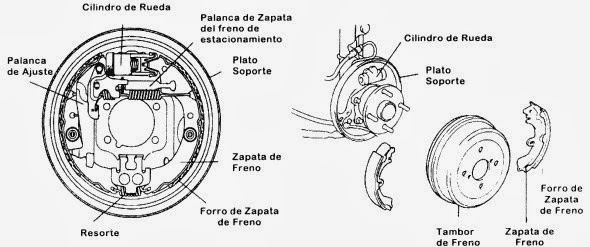
\includegraphics[width=0.65\textwidth]{./img_0009/freno_tambor.jpg}
\caption{Esquema de un freno de zapata interior}
\end{figure}
\item \textbf{Frenos de disco:} Consiste en un disco metálico de cierta anchura cuyo
centro está unido al elemento a frenar. En la mordaza o pinza de freno se
alojan las pastillas que, abrazando el disco metálico, lo frenan al actuar
sobre el

\begin{figure}[htbp]
\centering
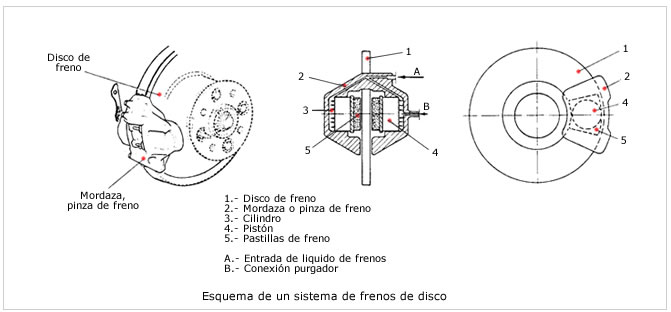
\includegraphics[width=0.9\textwidth]{./img_0009/freno_disco.jpg}
\caption{Esquema de un freno de disco}
\end{figure}
\end{enumerate}

\fbox{\parbox{\textwidth}{\textbf{Recuerda:} Los frenos, mediante el rozamiento,%
 permiten regular la velocidad de movimiento, bien disminuyéndola o manteniéndola.%
 Los frenos de zapata son muy utilizados en maquinaria}}
\section{Ruedas}
\label{sec:orgf783b5b}

Una rueda de neumáticos está constituida por:
\begin{itemize}
\item Un disco de acero sujeto con tornillos al plato del semi-palier
\item Una llanta metálica en cuya parte externa hay unas pestañas donde se alojan
los talones del neumático, y en su parte interna unas orejas para unir la
llanta al disco
\item El conjunto neumático montado sobre la llanta. Dado que las ruedas motrices y
directrices tienen misiones diferentes, sus neumáticos lo son en cuanto
tamaño, constitución y dibujo. A su vez el neumático está constituido por:
\begin{itemize}
\item Una \textbf{cámara} con forma de anillo hueco en la que queda encerrado el
aire. De esta manera el neumático amortigua las irregularidades de la marcha
\item Una \textbf{cubierta}. Básicamente esta compuesta por varias capas de
goma y otros materiales superpuestas y que van rodeando en los extremos unos
aros de acero colocados en los talones 

\begin{figure}[htbp]
\centering
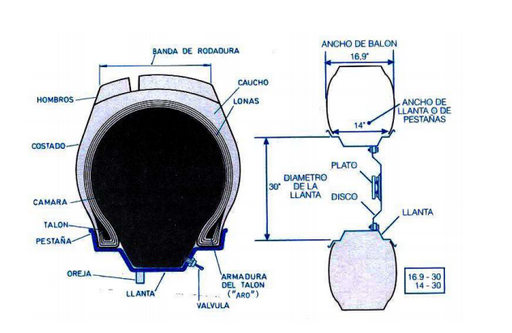
\includegraphics[width=0.6\textwidth]{./img_0009/esquema_rueda.PNG}
\caption{Elementos de una rueda}
\end{figure}
\end{itemize}
\end{itemize}


\begin{figure}[htbp]
\centering
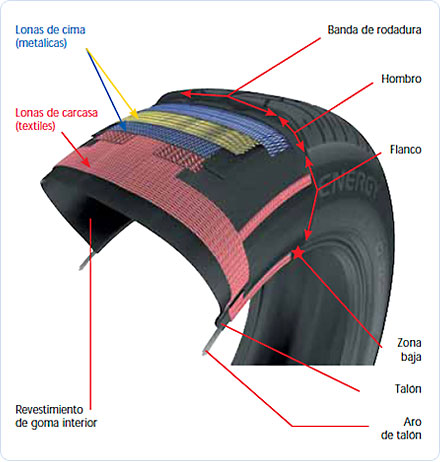
\includegraphics[width=0.55\textwidth]{./img_0009/neumatico1.jpg}
\caption{Partes de una cubierta de neumático}
\end{figure}

\section{Sistema eléctrico}
\label{sec:org0aebf7c}

Llamamos sistema eléctrico al conjunto de elementos que el tractor necesita
para realizar el arranque, encendido de luces u otras funciones para las que se
necesita corriente eléctrica. Los componentes básicos del sistema eléctrico son:
\begin{itemize}
\item \textbf{Batería de acumuladores:} es un generador de corriente eléctrica por medios
electroquímicos, es decir, transforma la energía eléctrica en energía química
y la almacena para después, cuando es necesario, reconvertirla en energía
eléctrica. Una batería de acumuladores se compone de una caja de material
aislante que guarda en su interior los elementos que hacen posible que la
energía se almacene y quede disponible. Estos elementos son una serie celdas
electroquímicas compuestas de unas placas de plomo sumergidas en un medio
líquido denominado electrolito. Sobre la tapa aparecen los bornes de plomo
correspondientes a los \uline{polos positivo (+) y negativo (-)}
 \begin{figure}[htbp]
\centering
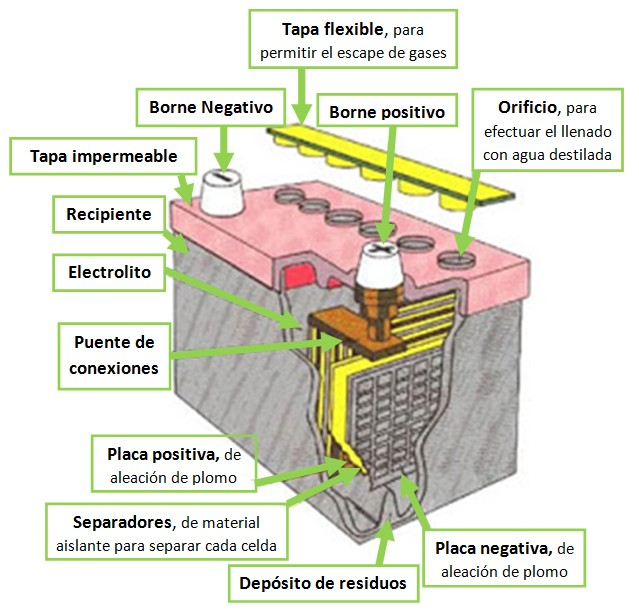
\includegraphics[width=0.7\textwidth]{./img_0009/bateria_partes.jpg}
\caption{Partes de una batería de acumuladores}
\end{figure}
 Cada celda de las baterias proporciona un voltaje de 2V. Según el número de
celdas la batería tendrá diferente voltaje. Hay baterías de 6V, 12V y 24V. La
capacidad de la batería se define por el \textbf{amperaje}, el valor de amperaje de
la batería será seleccionado de acuerdo al uso que se le vaya a dar.
\end{itemize}
\newpage
\begin{itemize}
\item \textbf{Alternador:} es el elemento que permite la recarga y el manteniento del
voltaje de la batería.

\begin{figure}[!ht]
\centering
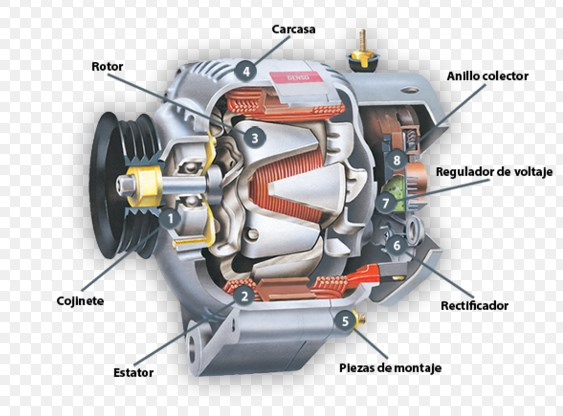
\includegraphics[width=0.7\textwidth]{./img_0009/alternador.jpg}
\caption{Alternador y sus partes}
\end{figure}
\end{itemize}

Un alternador consta de:
\begin{itemize}
\item Una parte fija llamada \textbf{estátor}, que lleva generalmente \textbf{tres bobinas}
\item Una parte móvil, el \textbf{rotor} con una sola bobina
\end{itemize}

Estas dos piezas forman una unidad y van recubiertas por dos tapas, en una de
ellas se montan las \textbf{escobillas} que son unos anillos por los que entra la
corriente continua. 

En esta misma tapa se van montados los \textbf{diodos rectificadores} que son los que
\uline{transforman la corriente alterna en continua} y de esta manera se \_puede
recargar la batería.

\recuerda{El alternador permite la recarga y el mantenimiento del voltaje de 
la batería}

\section{Puesto de conducción y cabina}
\label{sec:org2f25e8f}
En los actuales tractores se incluyen sistemas de ventilación, calefacción, aire
acondicionado, mandos ergonómicos, pantalla digital de control y un largo
etcetera.

La cabina proporciona \uline{aislamiento acústico} de ruidos y vibraciones, creando
unas buenas condiciones para trabajar de manera prolongada.

   \begin{figure}[htbp]
\centering
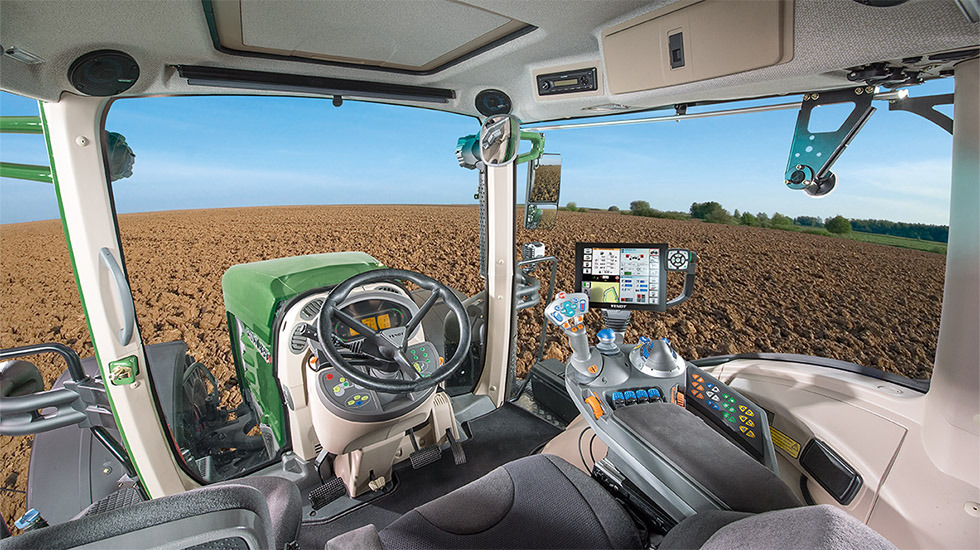
\includegraphics[width=0.7\textwidth]{./img_0009/cabina_tractor.jpg}
\caption{Interior de cabina}
\end{figure}
El \textbf{accidente} más común cuando se maneja un tractor son los \textbf{vuelcos}. Para
limitar las consecuencias debidas a los vuelcos los tractores deben ir
\uline{provistos de estructuras de protección} destinadas a detener el tractor sobre
un costado cuando este vuelca y \uline{reservar un espacio suficiente para que el 
conductor salga}. Estas protecciones \uline{son obligatorias para la comercialización 
de cualquier tractor}.
\newpage
Estas estructuras son:
\begin{itemize}
\item Arco o bastidor de dos postes: pueden ser delanteros o traseros
\begin{figure}[htbp]
\centering
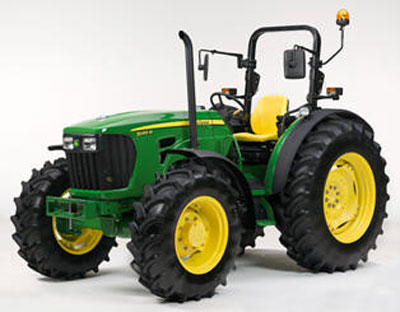
\includegraphics[width=0.6\textwidth]{./img_0009/bastidor2p.jpeg}
\caption{Bastidor dos postes}
\end{figure}

\item Cuadro, pórtico o bastidor de cuatro postes
\begin{figure}[htbp]
\centering
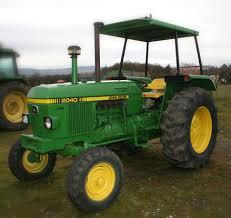
\includegraphics[width=0.6\textwidth]{./img_0009/bastidor4p.jpg}
\caption{Bastidor cuatro postes}
\end{figure}

\item Cabina
\begin{figure}[htbp]
\centering
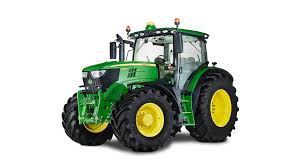
\includegraphics[width=0.6\textwidth]{./img_0009/cabina.jpg}
\caption{Cabina cerrada}
\end{figure}
\end{itemize}

\recuerda{Las estructuras de protección están destinadas a detener el 
tractor sobre un costado cuando éste se vuelca y \uline{reservar un espacio 
suficiente} para que el conductor salga indemne}

El asiento deberá estar situado de forma que no suponga peligro para el
acompañante ni obstaculice la conducción del tractor.

\uline{Deberá estar fijado \textbf{solidamente}} a alguno de los elementos de la estructura
del tractor.
\chapter{Mantenimiento básico de tractores y equipos de tracción}
\label{sec:org3e80d5d}

Con las labores de mantenimiento se consigue un ahorro económico y eficiencia de
los tractores y maquinaria empleados en la explotación. Para ello \textbf{es necesario}
realizar estas operaciones con \uline{la frecuencia indicada en los manuales} de estos
equipos. 

\section{Mantenimiento de máquinas y herramientas utilizadas en la explotación}
\label{sec:org65695b9}
Debido a que la maquinaría agrícola \uline{funciona bajo condiciones de trabajo muy
difíciles} (terreno y topografía desigual, exceso de polvo y lodo, temperaturas
extremas, etc) \textbf{es importante} realizar ciertas operaciones de mantenimiento
para obtener un \textbf{rendimiento adecuado} de los equipos.

Es importante comprobar el buen estado y funcionamiento de las condiciones
mecánicas ya que de ello \uline{no solo dependerá la calidad del trabajo}, sino
también el \textbf{confort y la seguridad del operario}.

\subsection{Mantenimiento preventivo}
\label{sec:org65f2f90}
Operaciones que se realizan \uline{para prevenir averías} sin que esto quiera decir
que nunca se van a presentar. 

Se trata de evitar riesgos y garantizar la seguridad del operador, a la vez que
reducimos costes innecesarios para la explotación agrícola.

\subsection{Mantenimiento correctivo}
\label{sec:orga07718d}
Consiste en cambiar o reparar las piezas que hayan sufrido un desperfecto por
averías imprevistas o haber cumplido su ciclo de trabajo.

Este tipo de mantenimiento, \uline{es mucho más costoso} y, por lo general, es
realizado por un mecánico.

Se denomina \textbf{programa de mantenimiento} a una serie de pasos \_destinados a
garantizar la vida útil de cualquier equipo o maquinaria desde el momento de la
adquisición hasta su fin. 
\recuerda{La \textbf{vida útil} es un intervalo de tiempo en el que un objeto puede cumplir correctmente con la función para la que ha sido diseñado}

Un buen programa de mantenimiento debe contener los siguientes aspectos:
\begin{itemize}
\item \textbf{Hoja de vida} de la máquina
\item Como se estructuran los controles de mantenimiento y asignación de las
diferentes responsabilidades a los operarios
\item Entrenamiento de operadores y operarios de mantenimiento básico
\end{itemize}

\subsection{Hoja de vida}
\label{sec:org07c7c98}
Debe incluir los siguientes apartados:
\begin{itemize}
\item \textbf{Identificación:} fecha de adquisición, marca, modelo, número de serie y
número de inventario interno
\item \textbf{Especificaciones:} manuales de operador y normas de fabricante
\item \textbf{Póliza de garantía:} garantiza el servicio gratuito por parte del fabricante
durante un período determinado de tiempo.
\item \textbf{Datos de distribuidores y concesionario:} nos proporcionan las asesorías de
mantenimiento \uline{preventivo}, así como las de mantenimiento
\uline{correctivo}. Conviene tener los datos de contacto (dirección, teléfono,
correo electrónico, fax.)
\item \textbf{Registros:} para recoger los datos relativos al \uline{mantenimiento de la
máquina}, asi como los de los \uline{combustibles, lubricantes, piezas y otros 
elementos empleados}.
\end{itemize}

En una hoja de vida bien estructurada \textbf{deben aparecer:}
\begin{itemize}
\item \textbf{Control de mantenimiento}
\item \textbf{Control de reparaciones}
\item \textbf{Control de consumo}
\item \textbf{Control de tiempo trabajado}
\end{itemize}

\subsection{Normas de seguridad en el mantenimiento y reparación}
\label{sec:org6641ca8}
Las \uline{normas básicas de seguridad} deben comprender los siguientes aspectos:
\begin{itemize}
\item Los trabajos de mantenimiento,reparación y limpieza, se deben realizar
\uline{únicamente} con la \uline{transmisión desconectada} y con el \uline{motor parado}. La
llave \uline{debe estar fuera} del contacto.
\item El apriete de tuercas y tornillos debe \uline{verificarse regularmente}. La
maquinaria agrícola se ve sometida a \uline{constantes vibraciones} por lo que es
muy conveniente realizar este tipo de comprobaciones y \uline{eventualmente volver a 
apretar tuercas y tornillos sueltos}.
\item En trabajos de mantenimiento con la \uline{máquina elevada} hay que \uline{prestar mucha 
atención a la seguridad} mediante los elementos apropiados.
\item Si utilizamos \uline{herramientas con filo}, emplearemos la herramienta \uline{apropiada 
al trabajo} y \uline{guantes}.
\end{itemize}

\recuerda{Un programa de mantenimiento es un conjuno de pasos que garantizan la vida
  util de cualquier equipo o maquinaria}


\section{Repercusiones económicas del mantenimiento}
\label{sec:orgb02d582}

El 70\% de los tractores agrícolas consume entre un \uline{10 y un 25\% más de lo 
necesario}, debido a un mal mantenimiento del tractor.

El mantenmiento debe realizarse \uline{durante toda la vida útil}, no solamente cuando
es nuevo o está en garantía.

Este mantenimiento \uline{debe ajustarse a las instrucciones del fabricante},
especialmente a lo que el motor se refiere.

El \textbf{manual del fabricante} debe leerse \uline{antes de poner en marcha el tractor} y
\textbf{consultarse} para la realización de reparaciones, regulaciones y mantenimiento,
pues en el \_vienen especificadas todas las revisiones que deberán realizarse.

Con el uso del tractor se produce una \uline{acumulación de suciedad en los filtros}
(polvo, hollín, etc.), desgastes y desajustes que \uline{incrementan el consumo de
combustible}.

\begin{center}%
\fbox{\parbox{\textwidth}{Por ello es \textbf{muy importante} para ahorrar del 
\textbf{10\% al 25\%} de combustible:}}
\end{center}

\begin{itemize}
\item \textbf{Leer} el manual de instrucciones
\item Mantener limpios los filtros de \textbf{aire} y de \textbf{gasoil}
\item Utilizar los \textbf{aceites} y \textbf{lubricantes} adecuados
\end{itemize}

\section{Operaciones de mantenimiento básicas}
\label{sec:orgf3c0e55}

\subsection{Sistema eléctrico}
\label{sec:orga2b5e1e}
La correcta rutina de mantenimiento del sistema eléctrico comprende los
siguientes puntos. Recuerda que debes \uline{seguir siempre} las instrucciones del manual:

\begin{itemize}
\item Si la batería \uline{no viene sellada} se debe comprobar semanalmente el nivel del electrolito
\item Limpieza y conservación de los terminales (a continuación detallamos los pasos
a seguir para realizar esta operación \uline{correctamente} y bajo \uline{condiciones de 
seguridad adecuadas}
\end{itemize}

\begin{enumerate}
\item \textbf{Limpieza de los bornes de la batería}
\label{sec:orgbb1d3cb}
\begin{enumerate}
\item \uline{Apagamos} el motor y sacamos la llave del contacto
\item Abrimos el capó y \uline{localizamos la batería}
\item Bajo el capó encontraremos la batería unida a dos cables, uno negativo (-) y
otro positivo (+) identificados por sus correspondientes signos en la  parte
superior de cada borne. \uline{Primero quitaremos el negativo} y luego el  positivo
utilizando la herramienta adecuada y \textbf{poniendo especial cuidado} en que, en
ningún caso, caigan sobre superficies metálicas y \uline{mucho menos que se toquen
entre ellos}.
\item Mezclar \textbf{bicarbonato sodico} y agua. Aproximadamente \uline{una cucharadita de 
postre con bicarbonato} por cada taza de agua.
\item \uline{Rociar} los bornes y los extremos de metálicos de los cables y \uline{dejar
actuar}
\item Tras unos minutos \uline{frotar suavemente} con un cepillo adecuado. (Los cepillos
metálicos pueden ser muy agresivos. \uline{Hay que emplearlos con cuidado para no 
dañar ningún elemento})
\item Aclarar con agua y secar
\item Por último aplicar \textbf{vaselina} a los bornes para retrasar la corrosión. Una
vez hecho esto conectamos los cables a los bornes \uline{primero el polo \textbf{positivo}}
y después el \textbf{negativo}
\end{enumerate}
\end{enumerate}

\subsection{Sistema de alimentación}
\label{sec:org4e06d06}

La importancia de un \uline{adecuado mantenimiento} se basa en obtener un \uline{bajo consumo}
de combustible, y \uline{bajas emisiones contaminantes} (humo negro, oxidos nitrosos,
monóxido de carbono,etc).

Un adecuado protocolo de actuación incluye:

\begin{itemize}
\item Asegurar que el combustible que se suministra está en \uline{condiciones optimas}
\begin{itemize}
\item Almacenar el combustible bajo techo con el fin de posibilitar la eliminación
de impurezas y el agua de condensación y \uline{que no entre agua de lluvia en los tanques}.
\item \uline{Evitar} la utilización de embudos y recipientes de trasvasar
\end{itemize}
\item Llenado del tanque de combustible al \uline{final de cada jornada de trabajo}
\item Cambio de filtro según las indicaciones del fabricante
\end{itemize}

\recuerda{El principal cuidado que hay que dar a la \textbf{bomba de inyección} 
es la limpieza del filtro, ya que si se llena de impurezas puede dañar este elemento} 

\subsection{Sistema de refrigeración}
\label{sec:org07c1049}
Para realizar un correcto mantenimiento del sistema de refrigeración \uline{por agua}
se debe:
\begin{itemize}
\item Utilizar \uline{unicamente} líquido adecuado. Esto es, liquido \emph{anticongelante} que
lleva aditivos para \uline{evitar la corrosión}.
\item Revisar el nivel de agua del radiador \uline{cada jornada de trabajo}
\item Controlar la tensión de la correa del ventilador y su estado
\item Mantener limpio el radiador. \textbf{Precaución} al utilizar \uline{aire comprimido} para
la limpieza del radiador pues se pueden dañar las \uline{aletas deflectoreas}
\end{itemize}

\subsection{Sistema de engrase}
\label{sec:org881234e}

Una correcta lubricación \uline{prolonga la vida útil} del motor. El mantenimiento
adecuado consiste en:
\begin{itemize}
\item Usar siempre aceite limpio y del tipo indicado en el manual
\item \uline{Antes de comenzar} la jornada de trabajo hay comprobar que el \uline{nivel de 
aceite está al nivel correcto}
\item Realizar el cambio de aceite y del filtro \uline{según las indicaciones del
fabricante}
\end{itemize}

A continación damos unas recomendaciones para la comprobación del \uline{nivel de aceite}:
\begin{enumerate}
\item \textbf{Comprobación del nivel de aceite:}
\label{sec:orgc27b449}
\begin{enumerate}
\item Asegurarse de que \textbf{antes} de medir el aceite , el tractor está en \uline{horizontal}
con \uline{motor parado y en frío}. Si comprobamos el nivel con el motor en caliente
podemos obtener un \uline{error en a medición} ya que por la dilatación de los
materiales puede marcar más de lo que tenemos en realidad.
\item Al coger la varilla de medición comprobarás que la \uline{parte del mango tiene un 
color diferente} al resto para diferenciarlo. La varilla tiene dos muescas en
su extremo que marcan el nivel \uline{máximo y el mínimo}.
\item Extraer la varilla del depósito de aceite con suavidad y \uline{limpiarla con un
trozo de trapo o un trozo de papel}.
\item \uline{Introducimos de nuevo la varilla y la extraemos}.
\item En esta medición el aceite debe estar \uline{entre las dos muescas} para que el
nivel de aceite \textbf{sea el correcto}
\end{enumerate}
\end{enumerate}

\subsection{Sistema de transmisión}
\label{sec:org3aaf63b}

Podemos realizar las siguientes acciones:
\begin{itemize}
\item Controlar el nivel de aceite de la caja de cambio
\item Verificar que el embrague funciona correctamente
\item Cambiar el aceite de la caja de cambio como lo indique el manual
\end{itemize}

\subsection{Sistema hidráulico}
\label{sec:orgdd36162}

Tenemos los siguientes procedimientos:
\begin{itemize}
\item Verificación diaria del nivel de fluido
\item Emplear \uline{unicamente} el tipo de aceite que recomienda el fabricante
\item Cambiar el filtro con la frecuencia que indique el manual de instrucciones
\end{itemize}

\chapter{Prevención de riesgos laborales con maquinaria}
\label{sec:org5aafcba}

A continuación vamos a describir en líneas generales los riesgos más comunes a
diversa maquinaria y entender las razones por las cuales determinados mecanismos
son peligrosos. 

\vspace{1cm}
\noindent
\fbox{%
\begin{minipage}{\textwidth}%
El agricultor toma ciertos riesgos que están relacionados con la naturaleza 
del trabajo que realiza. Las causas más habituales de los accidentes laborales
son:
\begin{itemize}
\item Que el operario/agricultor trabaja solo
\item Que trabaja con maquinaria desde edades tempranas, lo que causa un exceso
      de relajación cuando está usandola
\item Que el trabajo se realiza de forma intensiva. Se acumulan muchas horas de 
      trabajo en largas jornadas, por lo que el cansancio aumenta
\item La escasa capacitación y formación profesional
\end{itemize}
\end{minipage}} 

\section{Reconocimiento de los riesgos y peligros más comunes en maquinaria agricola}
\label{sec:orge4d2fb0}

En la utilización de cualquier tipo de maquinaria agricola existen unas
\uline{disposiciones mínimas en seguridad y salud} establecidas en el \textbf{Real Decreto 
1215/1997} (modificado por el Real Decreto 2177/2004), por el que se establecen
las disposiciones mínimas de seguridad y salud para la utilización por los
trabajadores de los equipos de trabajo:
\begin{itemize}
\item \uline{Debe existir} un dispositivo de \textbf{parada total}
\item La parada \uline{debe cortar el suministro de energía} a los organos de accionamento
\item Los organos de accionamiento \_deben estar señalizados y ser claramente
visibles.
\end{itemize}

Las \textbf{áreas de riesgo} comunes a cualquier máquina agrícola son:
\begin{itemize}
\item \textbf{Engranajes}. Deben estar \uline{siempre protegidos} y \textbf{no} desmontar ni reparar con la
máquina en marcha
\item \textbf{Puntas, aristas de corte y cizallamiento}. \uline{Siempre protegidas} y repararse
\uline{siempre con la máquina parada}.
\item \textbf{Ejes y puntos giratorios de arrollamiento} deben estar \uline{protegidos en su
totalidad} sobre todo en sus extremos
\item Los \textbf{puntos de arrastre} sobre todo en cosechadoras y empacadoras \uline{NUNCA}
deben ser manpulados con la máquina en marcha
\item \textbf{Puntos de aplastamiento} sobre todo cuando se realizan operaciones de
\uline{manipulación de cargas} y \uline{acople de aperos}
\item Por último las \textbf{proyecciones} debidas a partículas de madera, tallos, piedras
de pequeño tamaño, etc., escupidas por elementos que giran a gran
velocidad. Siempre que sea posible las \_máquinas contarán con carcasas
protectoras y si no, se emplearán los correspondientes \uline{equipos de
protección individual}
\end{itemize}

\recuerda{Las áreas de riesgo comunes a cualquier máquina agricola son: los engranajes, 
puntas y aristas de corte y cizallamiento, ejes y puntos giratorios de arrollamiento,
puntos de arrastre, puntos de aplastamiento y las proyecciones}

\begin{enumerate}
\item \textbf{Puntos de engranaje:}
\label{sec:org4cc2895}

Es la \uline{zona donde dos o más elementos entran en contacto}, estando al menos un
de ellos en movimiento.

La forma más habitual de accidente es el \uline{atrapamiento} de la mano, pie u otra
parte del cuerpo o de vestimenta.

Las \textbf{medidas de prevención} en estos puntos son:
\begin{itemize}
\item Dichos puntos deben estar convenientemente protegidos
\item \uline{No operar} la maquinaria si dichas protecciones no están colocadas
\item \uline{Conocer los puntos peligrosos}, localizarlos y evitar aproximarse a ellos
cuando la máquina esté en funcionamiento
\item \uline{No realizar ninguna intervención} cuando la máquina o alguna de sus partes
esté en movimiento
\end{itemize}

\begin{figure}[htbp]
\centering
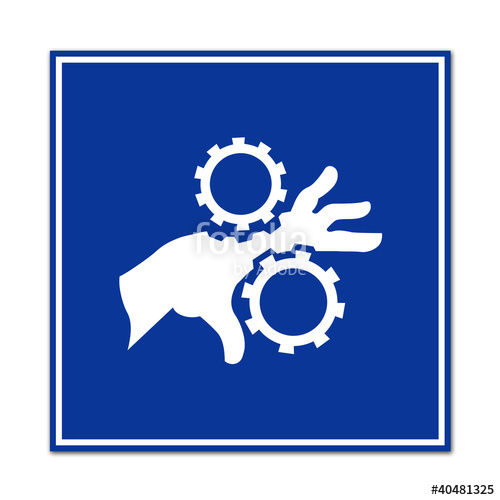
\includegraphics[width=0.8\textwidth]{./img_0009/riesgo_engranaje.jpg}
\caption{Componentes del tractor}
\end{figure}

\item \textbf{Puntos de cizallamiento - Zonas cortantes:}
\label{sec:org105b774}

Son puntos o zonas de corte en las extremidades de dos objetos que se mueven en
la misma dirección y sentido opuesto, o cuando dos objetos pasan relativamente
cerca uno del otro para cortar materiales más o menos blandos.

\uline{Los accidentes pueden ser producidos por:}

\begin{itemize}
\item Elementos construidos para efectuar una \textbf{acción cortante}, por ejemplo una
barra de corte de una podadora
\item \textbf{Herramientas manuales} dotadas o no de motor. Motosierra, desbrozadora,
hacha, tijera de podar, etc
\end{itemize}

\recuerda{Es importante conocer todos los puntos peligrosos, localizarlos en la 
máquina y evitar aproximarse a ellos cuando la máquina está en funcionamiento}

\uline{Las medidas de prevención} son:

\begin{itemize}
\item Las zonas de corte \uline{deben estár protegidas}
\item \uline{Nunca y bajo ninguna circunstancia}, nadie se debe colocar en el área de
acción de la máquina
\item \uline{Alejarse} de las zonas cortantes cuando estas estén en movimiento
\end{itemize}

\begin{figure}[htbp]
\centering
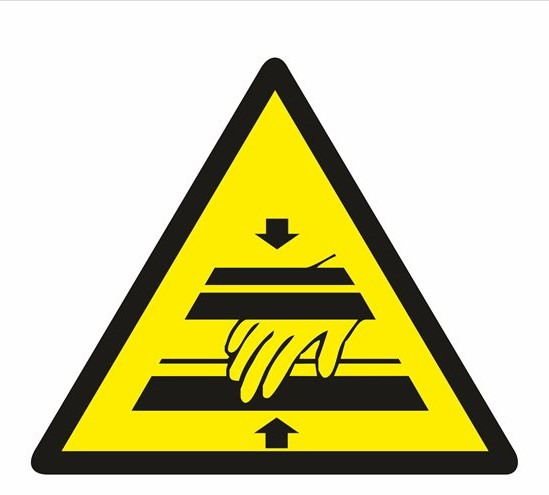
\includegraphics[width=0.8\textwidth]{./img_0009/corte_mano.jpg}
\caption{Pictograma de riesgo de corte}
\end{figure}

\recuerda{Se deben montar los dispositivos de seguridad en caso de que hayan 
sido retirados, tras efectuar un ajuste o reparación}

\item \textbf{Puntos de atrapamiento o enganche:}
\label{sec:org9225098}

El atrapamiento \uline{se produce} cuando una persona o parte de su cuerpo es
\uline{enganchada o aprisionada} por mecanismos de las máquinas o entre objetos,
pìezas o materiales.

Los accidentes por atrapamiento \uline{comienzan} por el \textbf{arrastre de un hilo} u orta
parte abierta de la vestimenta, que rota o abierta, se enrosca en torno a un eje
rotatorio. 

\begin{figure}[htbp]
\centering
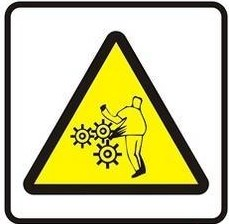
\includegraphics[width=0.8\textwidth]{./img_0009/atrapamiento.jpg}
\caption{Pictograma de riesgo de atrapamiento}
\end{figure}

Las puntas de ejes salientes \_también pueden enganchar las vestimentas.

La ropa, \uline{que generalmente es bastante resistente}, puede aguantar estos
enganches y el operario \uline{no la puede romper}. De esta manera se \textbf{enrrolla
rápidamente} y el operario es violentamente arrastrado hacia el mecanismo que
gira. 

Las \textbf{lesiones} que se pueden producir por este tipo de accidentes puedn ser
desde \uline{contusiones leves} (golpes suaves) a \uline{lesiones graves como amputaciones}
e incluso \textbf{mortales}.

Accidentes de este tipo también pueden ocurrir a \uline{quien lleva el pelo largo sin
recoger}. El pelo puede quedar prendido y enrollado en las partes giratorias
produciendose \textbf{heridas graves y permanentes}.

\item \textbf{Zonas de aplastamiento:}
\label{sec:orgdf52b36}

Los accidentes de este tipo pueden ser \uline{voluntarios o involuntarios} (por
desplazamiento de una carga) y se deben a \uline{la caida de objetos} o materiales
durante la ejecución de trabajos, o en \uline{operaciones de transporte y elevación}.

Se pueden prducir las \textbf{siguientes situaciones:}
\begin{itemize}
\item Situarse \uline{debajo de productos apilados}
\item Situarse \uline{debajo de cargas suspendidas}
\item En acciones de \uline{acoplamiento y desenganche de aperos}
\item \uline{Traslado manual de objetos pesados}
\item Operaciones de \uline{mantenimiento} bajo maquinaria \textbf{insuficientemente} sujeta
\item Operaciones \uline{debajo de cargas basculantes} en posición elevada
\end{itemize}

\begin{figure}[htbp]
\centering
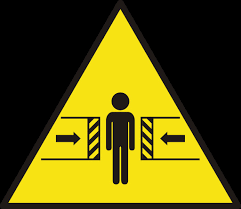
\includegraphics[width=0.8\textwidth]{./img_0009/aplastamiento.png}
\caption{Pictograma riego aplastamiento}
\end{figure}

\begin{enumerate}
\item \textbf{Medidas de prevención para atrapamiento y aplastamiento:}
\label{sec:orgc183061}

Se producen en los mecanismos en movimiento del tractor, principalmente:
\begin{itemize}
\item \textbf{Toma de fuerza y eje cardánico}
\begin{itemize}
\item Al conectar la toma de fuerza  \uline{nadie debe permanecer cerca} al eje en
movimiento
\item No conectar \textbf{nunca} la toma de fuerza con el motor parado
\item No permitir que nadie con \uline{ropas sueltas o colgantes} se acerque demasiado a
la toma de fuerza
\item Antes de accionar la toma de fuerza hay que \uline{comprobar si el número de
revoluciones} se corresponde con el permitido para la máquina
\item Utilizar \uline{únicamente} el eje cardánico para la máquina que prevee el
fabricante, con su correspondiente dispositivo de seguridad
\item \uline{Evitar} que el cardan permanezca enganchado a la toma de fuerza por un
extremo y que \uline{descanse en el suelo por el otro}
\end{itemize}
\end{itemize}
\recuerda{Los accidentes por atrapamiento pueden comenzar por el arrastre de un hilo 
u otra parte abierta de la vestimenta}
\begin{itemize}
\item \textbf{Protector de la toma de fuerza}
\begin{itemize}
\item Al desmontar el cardan hay que fijar la cubierta protectora de la toma de fuerza
\item Debe utilizarse el escudo protector de la toma de fuerza \_en los momentos de
enganche, desenganche y mientras se está utilizando
\item Es \uline{completamente desaconsejable} utilizar el escudo protector para subirse
al tractor, o apoyarse en el en las maniobras de enganche y desenganche, y
\uline{mucho más aún} ir subido a el con el tractor en marcha
\end{itemize}
\item \textbf{Enganche tri-puntal}
\begin{itemize}
\item Antes de montar y desmontar aperos en el enganche, hay que \uline{situar los  
mandos de manera conveniente} para que no se puedan accionar de \uline{manera 
involuntaria}.
\item Al accionar el mando del enganche no hay que situarse \uline{nunca} entre el
tractor y la máquina
\item Los cables de desenganche en los enganches rápidos \uline{deben colgar sueltos} y
no deben desengancharse solos en la posición baja
\item \uline{Bloquear} la palanca de accionamiento del descenso en el transporte por
carretera
\end{itemize}
\item \textbf{Sistema hidraulico}
\begin{itemize}
\item El accionamiento debe hacerse \uline{siempre desde una posición segura}
\item Al conectar manguitos de sistemas hidráulicos se debe prestar atención a la
\uline{conexión reglamentaria}
\item Controlar el \uline{deterioro y envejecimiento de los tubos}
\end{itemize}
\end{itemize}

\recuerda{Nadie, bajo ningúna circunstancia, se debe colocar dentro del área de 
acción de la máquina}
\end{enumerate}
\end{enumerate}

\section{Tractores: protectores de vuelco del tractor}
\label{sec:org8159e98}

El riesgo de \textbf{vuelco} es el accidente más común e importante con el tractor, por
la gravedad de las lesiones que se producen cuando ocurre.

Durante su utilización deberían conocerse todas las posi-bles causas de vuelco y
los factores que pueden aumentar la gravedad de las lesiones. Para la
identificación del peligro de vuelco deben considerarse las características del
tractor, de los equipos acoplados, del entorno de trabajo y del conductor, así
como la interacción entre ellas. 

El \uline{daño más grave} derivado del accidente por vuelco es la \textbf{muerte} del conductor
por aplastamiento si el tractor no  dispone  de  la \textbf{estructura  de  protección} 
en  caso  de  vuelco y el \textbf{cinturón de seguridad}. Dicha estructura  \uline{no  
reduce  la  probabilidad de  vuelco}  sino  que  está  diseñada para \uline{minimizar  
la gravedad de las lesiones} si ocurriera el accidente. También pueden
presentarse lesiones si el tractor dispone de estructura de protección pero  el
conductor  \uline{no  lleva  puesto  el  cinturón  de  seguridad} que lo mantiene
dentro de los límites de la zona de seguridad garantizada por la estructura de
protección. 

Por otro lado, las lesiones pueden empeorar debido a que se acumula un
importante \uline{tiempo de retraso hasta que el accidentado es localizado}, ya que
estos accidentes suelen ocurrir en lugares apartados de las explotaciones
agrarias 

\section{Tipos de vuelco del tractor agrícola}
\label{sec:orgb6f9b0c}
\subsection{Vuelco lateral del tractor}
\label{sec:org8b810fb}

\begin{figure}[htbp]
\centering
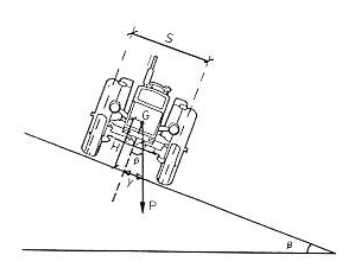
\includegraphics[width=.9\linewidth]{./img_0009/vuelco_lat_graf.PNG}
\caption{}
\end{figure}

Este tipo de vuelco supone el 90\% de los casos. Va a depender de:
\begin{itemize}
\item La pendiente del terreno \(\beta\)
\item La altura del centro de gravedad \emph{H}
\item La anchura de la via \emph{S}
\end{itemize}

En los dos primeros parámetros (\(\beta\) y \emph{H}), \uline{al aumentar su valor aumenta el 
riesgo de vuelco}. 

En la anchura de vía \emph{S}, es al contrario, a \uline{mayor anchura menor riesgo}.

Los \textbf{contrapesos delanteros} hacen \uline{descender el centro de gravedad} y por tanto
el riesgo de vuelco.
\begin{figure}[htbp]
\centering
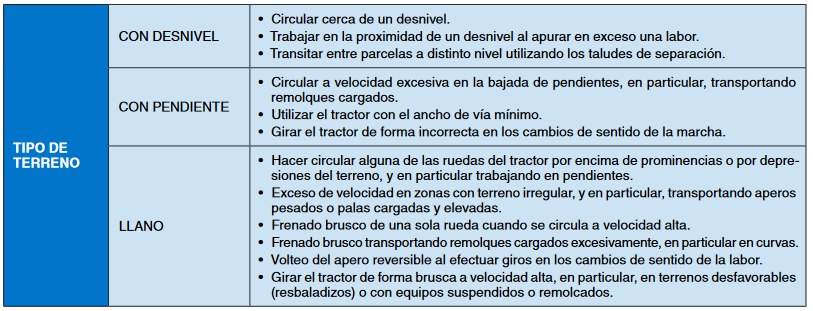
\includegraphics[width=\textwidth]{./img_0009/vuelco_lat.PNG}
\caption{Vuelco lateral (actos inseguros o maniobras incorrectas)}
\end{figure}
\subsection{Vuelco hacia atras}
\label{sec:orgd4dfce5}

\begin{center}
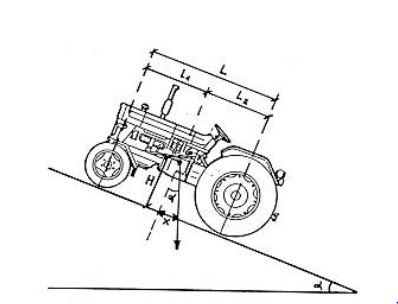
\includegraphics[width=.9\linewidth]{./img_0009/vuelco_atras_graf.PNG}
\end{center}

Es mucho \uline{menos frecuente que el lateral}.

Va a depender de:
\begin{itemize}
\item La inclinación del terreno \(\alpha\)
\item La altura del centro de gravedad \emph{H}
\item La distancia de \emph{H} al eje trasero \emph{L\(_{\text{2}}\)}
\end{itemize}

En los dos primeros, al \uline{aumentar su valor aumenta el riesgo}.

El \uline{lastrado delantero} con contrapesos, reduce el riesgo al reducir la altura
del centro de gravedad, y aumentar el par contrario al vuelco

\subsection{Vuelco con aperos}
\label{sec:org1000d49}
\begin{center}
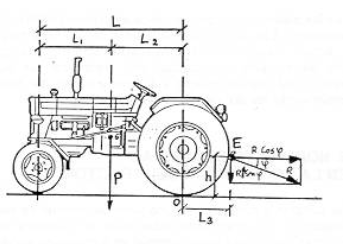
\includegraphics[width=.9\linewidth]{./img_0009/vuelco_aperos.PNG}
\end{center}

Entendemos por apero \uline{cualquier elemento unido o acoplado al tractor}.

Va depender de: 
\begin{itemize}
\item La posición del centro de gravedad (si está bajo y adelantado se disminuye
el riesgo)
\item El peso del apero y la fuerza de tiro (al aumentar, aumenta el riesgo)
\item El punto de enganche del apero (cuanto más alto, más riesgo)
\end{itemize}
\end{document}